\documentclass[ngerman={babel}, utf8, bigger, t, xcolor={table,dvipsnames}, ompress, hyperref={bookmarks,colorlinks},red]{beamer}

\usepackage{pgfpages} %used for pdfpres two-window output

\usepackage{tikz}	%graphics
\usetikzlibrary{positioning}	%easier positioning
\usepackage{tikz-uml}	%UML diagrams

\title[Embedded Systems]{Software Engineering in Embedded Systems}
\author{Stephan Heidinger}
\date{19. January 2012} %hier Datum des Vortrags einfügen
\institute[Seng-Seminar]{Seminar: Software Engineering \\ Fachbereich für Informatik und Informationssysteme \\ Universtität Konstanz}

\usetheme{AnnArbor}
%\useoutertheme{sidebar2} %logo einbauen?
\usepackage{sidebar}
%\useinnertheme{circles}
%\usecolortheme{albatross}	%nice dark (blue) %not feasible with notes
\usecolortheme{dolphin}	%nice blue around, light inside
%\usecolortheme{beetle}	%nice, dark around, almost light inside
\pgfdeclareimage[height=1.925cm]{uni-logo}{logo}%[height=0.5cm]{university-logo}{images/uni_logo}
\logo{\pgfuseimage{uni-logo}}
\setbeamercolor{structure}{fg=black}%,bg=black!75}
\setbeamercolor{frametitle}{fg=white}
%\setbeamercolor{title in sidebar}{fg=yellow,bg=green}

%\usecolortheme{}
%\useinnertheme{}
%\useoutertheme{}
%\usefontheme{}

%standardoverlayreihenfolge: aktuelles overlay und auf allen danach
\beamerdefaultoverlayspecification{<+->}
%dasselbe + highlight auf dem aktuellen
%\beamerdefaultoverlayspecification{<+-| alert@+>}
%unsichtbarer text ist halb sichtbar
\setbeamercovered{transparent=25}
%show note-slides
\setbeameroption{show notes}
%\setbeameroption{show notes on second screen=right} %use impressive, both monitors same resolution...
\setbeameroption{show notes on second screen=left} %use impressive, both monitors same resolution...

\begin{document}
%colors for definition boxes
\setbeamercolor{defHeader}{fg=black,bg=red!80}
\setbeamercolor{defBody}{fg=blue,bg=red!40}
%colors for tables
\rowcolors{1}{black!20}{black!40}

\AtBeginSection{% This will post whatever is inside at the beginning of each section, maybe use sidebar instead
	\begin{frame}<beamer>{Outline}%nur für beamer, nicht für handout
	\addtocounter{framenumber}{-1}
	\tableofcontents[currentsection]
	\end{frame}
}

\frame[plain]{\titlepage}
%\begin{frame}{}{}% Beginn der Titelfolie
%\maketitle
%\end{frame}% Ende der Titelfolie

%\section{Motivation}
\begin{frame}{Embedded Systems - What's that? - I}
	\begin{beamerboxesrounded}[upper=defHeader, lower=defBody,shadow=true]{Definition}
	\emph{``An \textbf{embedded software system} is part of a hardware/software system that reacts to events in its environment. The software is `embedded' in the hardware. Embedded systems are nominaly real-time systems.''\\
		{\tiny Software Engineering, p.561, Edited by Ian Sommerville, Ninth Edition}} %bibliography
	\end{beamerboxesrounded}
	\note<.>{``An \textbf{embedded software system} is part of a hardware/software system that reacts to events in its environment. The software is `embedded' in the hardware. Embedded systems are nominaly real-time systems.''}
	\note<.>{\\ explanation NEXT SLIDE}
\end{frame}

\begin{frame}{Embedded Systems - What's that? - II}
	\begin{itemize}
		\item Embedded Systems: \dots
		\begin{itemize}
			\item \dots respond to physical world
			\note<.>{respond to physical world}
			\item \dots respond in real time (``have a \emph{deadline}'')
			\note<.>{resüpm om real time \\
			(``have a deadline'') $\to$ time in which the result is produced}
			\item \dots often have little resources
			\note<.>{often have litte resources \\ i.e. not `computers'}
			\item \dots run on special purpose hardware
			\note<.>{run on special purpose hardware}
			\item \dots run in real-time operating system
			\note<.>{run in real time operating systems}
		\end{itemize}
	\end{itemize}
\end{frame}

\begin{frame}{Embedded Systems - What's that? - III}
	\begin{itemize}
		\item Examples for Embedded Systems:
		\begin{itemize}
			\item airbag
			\note<.>{\textbf{airbag:}\\ strict deadline \\ catastrophic result on failure}
			\item cell phone / `modern' phone
			\note<.>{\textbf{cell phone:}\\ phone must be answered before call quit vom other side}
			\item burglar alarm
			\note<.>{\textbf{burglar alarm:}\\ }
			\item (fully automatic) coffee machine
			\note<.>{\textbf{coffee machine:}\\ dont want to have coffee, when its cold...}
			\item danger detection %(NPP, earthquake, \dots)
			\note<.>{\textbf{danger detection:} \\ earthquake, toxins, \dots \\ depending on the kind of danger, absolutely no time to spare.}
			\item \dots
			\note<.>{One can produce more examples on a whim \\ especially in cars}
		\end{itemize}
	\end{itemize}
\end{frame}

\begin{frame}{Motivation}
	\begin{itemize}
		\item We see:
		\note<.>{We see:}
		\begin{itemize}
			\item Embedded Systems are everywhere!
			\note<.>{Embedded Systems are everywhere!}
			\item There are probably more Embedded Systems than computers out there!
			\note<.>{There are probably more Embedded Systems than computers out there!}
		\end{itemize}
		\item We realize:
		\note<.>{We realize:}
		\begin{itemize}
			\item Man, they must be important.
			\note<.>{they must be important.}
			\item There sure is some money in this.
			\note<.>{there sure is some money in this}
			\note<.>{\\ \textbf{some money:}\\ C-programing \\ special skills}
			\only<7>{\item I did an internship producing an embedded system.}
			\note<.>{and i did an internship producing an embedded system at PSI \\ monitoring device for the detector of an particle accelerator}
		\end{itemize}
		\end{itemize}
\end{frame}

%\section*{Outline}
\begin{frame}<beamer>{Outline}
\addtocounter{framenumber}{-1}
\tableofcontents
\note<.>{this is the structure of my talk: \\ embedded systems DESIGN \\ architectural patterns \\ timing analysis \\ real-time operating systems}
\end{frame}

\section{Embedded Systems Design}
\begin{frame}{Problems}
	\begin{itemize}
		\item Problems in embedded Systems:
		\note<.>{several problems in emb-systems that are not in ``normal'' systems}
		\begin{itemize}
			\item deadlines
			\note<.>{\textbf{deadlines:} every process has deadline until result must exist \\ hard systems: deadline not met, failure\\ soft system: deadline not met, bad results}
			\item environment
			\note<.>{\textbf{environment:}\\ is unpredictable \\ embedded Software $\Rightarrow$ must be concurrent}
			\item continuity
			\note<.>{\textbf{continuity:}\\ embedded Software $\Rightarrow$ does not normally terminate \\ software has to be reliable \\ may need update while operating}
			\item direct hardware interaction
			\note<.>{\textbf{direct hardware interaction:}\\ uncommon hardware (i.e. detonator in airbag) \\ speed issues (hardware is faster than software)}
			\item safety \& reliability
			\note<.>{\textbf{safety \& reliability:}\\ cost of failure high \\ either economical or in human life}
		\end{itemize}
	\end{itemize}
\end{frame}

\begin{frame}{Embedded Systems Design}
	\begin{itemize}
		\item design steps
		\note<.>{\textbf{design steps}\\ not all are necessary, but most will be. \\ no definite order}
		\begin{itemize}
			\item platform selection
			\note<.>{\textbf{Platform selection:}\\ what hardware? \\ choice of Real-time operating system {\tiny (later)} \\ power consumption (mobile device, backup)}
			\item special purpose hardware
			\note<.>{\textbf{special purpose hardware:}\\ What is to be implemented in software, what in hardware \\ do we need uncommon hardware? \\ design special hardware? \\ replace software by hardware?}
			\item stimuli:
			\note<.>{think about \textbf{stimuli:}\\ describe behavior of system by listing received stimuli and reactions \\ stimuli = signals \\ often: stimulus $Rightarrow$ defined response \\ \vspace*{2em} example AFTER THIS SLIDE}
				\begin{enumerate}
					\item periodic stimuli
					\note<.>{\textbf{periodic stimuli:}\\occur at predictable intervals \\ predefined reaction per stimulus \\ i.e. polling}
					\item aperiodic stimuli
					\note<.>{\textbf{aperiodic stimuli:}\\ occurr irregularly and unpredictably \\ often interrupts \\ i.e. alarms, failures, IO operation finished, etc}
					\note<.>{\textbf{stimuli list:}\\best practice: stimuli list with \textbf{all} stimuli. \\ \vspace*{2em} example AFTER THIS SLIDE}
				\end{enumerate}
			\item Timing analysis
			\note<.>{\textbf{Timing analysis:}\\ For each stimulus and response $\Rightarrow$ find timing constraints \\ timing constraints $\Rightarrow$ deadlines}
			\item Process design
			\note<.>{\textbf{Process design:}\\ aggregate the stimuli \& responses into concurrent processes \\
			SEE Architectural patterns}
			\item Algorithm design
			\note<.>{\textbf{Algorithm design:}\\ For each stimulus \& response $\Rightarrow$ design algorithm \\ especially important for computationally intensive tasks (signal processing) \\ Do we need to implement these in hardware? (i.e. control systems)}
			\item Data design
			\note<.>{\textbf{Data design:}\\ How to store data, that will be exchanged \\ semaphore \& critical regions \& monitors \& \dots}
			\note<.>{\\ \vspace*{2em} \textbf{circular buffer:} producer \& consumer may run at different speeds}
			\item Process scheduling
			\note<.>{\textbf{Process scheduling:}\\ ensure, that processes meet their deadline}
			\note<.>{\ \\ \vspace*{2em} \textbf{all shown:}\\ not all need to be done, but most probably will \\ which \& order depends on what we design }
			\note<.>{\\ \vspace*{1em} \textbf{after this design steps:}\\ make sure system can meet deadlines \\ static analysis \\ simulation
			}
		\end{itemize}
	\end{itemize}
\end{frame}

\begin{frame}{Example: radiation warning system}
	%\usetikzlibrary{positioning}
\begin{tikzpicture}
%shielding
\only<2->\draw (-.1,-.1) rectangle (6.1,6.1);
%reactor
\only<2->\draw[fill] (3,3) circle (1);
\only<2->\node[draw,circle,fill] (reactor-icon) at (6.5,5.8) {};
\only<2->\node (reactor) [right=0cm of reactor-icon] {reactor};

%room 1
\only<3->\draw (0,3) rectangle (3,6);
\only<3->\node (room1) at (1.5,4.5) {room 1};
\only<4->\draw[fill=blue!75] (2.5,5) circle (.1);
\only<4->\draw[fill=blue!75] (1,3.5) circle (.1);
%room 2
\only<3->\draw (0,0) rectangle (3,3);
\only<3->\node (room1) at (4.5,4.5) {room 2};
\only<4->\draw[fill=blue!75] (3.5,5) circle (.1);
\only<4->\draw[fill=blue!75] (5,3.5) circle (.1);
%room 3
\only<3->\draw (3,3) rectangle (6,6);
\only<3->\node (room1) at (1.5,1.5) {room 3};
\only<4->\draw[fill=blue!75] (2.5,1) circle (.1);
\only<4->\draw[fill=blue!75] (1,2.5) circle (.1);
%room 4
\only<4->\draw[fill=blue!75] (3.5,1) circle (.1);
\only<4->\draw[fill=blue!75] (5,2.5) circle (.1);
\only<3->\draw (3,0) rectangle (6,3);
\only<3->\node (room1) at (4.5,1.5) {room 4};

%legend
\only<4->\node[draw,circle,fill=blue!75] (sensor-icon) at (6.5,5.3) {};
\only<4->\node (reactor) [right=0cm of sensor-icon] {sensor};

%legend-border
\only<2->\draw (6.2,5) rectangle (8.2,6.1);
\end{tikzpicture}
\end{frame}

\begin{frame}{Example: Stimuli-List of a radiation warning system}
	\setbeamercovered{invisible}
	\begin{tabular}{p{9em}p{13em}}
		\rowcolor{structure.fg}\hline \textcolor{white}{Stimulus} & \textcolor{white}{Response} \pause \\
		single sensor positive & flash yellow light around sensor \pause \\
		both sensors in one area positive & flash red light in area, sound acoustic alarm in area \pause \\
		Voltage drop of 10-20\% & switch to backup power; run power supply test \pause \\
		Voltage drop of more than 20\% & switch to backup; run power supply test; call technician \\
	\end{tabular}
	\note<1>{Now we built a list of stimuli and responses}
	\note<2>{single sensor positive \\ want to warn people, that there is something \\ flash a yellow light around the sensor}
	\note<3>{two sensors in one are positive \\something is really wrong \\ flash red light in are \\ sound alarm}
	\note<4>{small voltage drop \\ probably nothing bad \\ switch to backup power \\ run power supply test}
	\note<5>{big voltage drop \\ do the same as on small drop \\ call technician}
	\note<5>{\ \\ \textbf{LAST CELL:}\\}
	\setbeamercovered{transparent=25}
\end{frame}



\begin{frame}{Embedded system modeling}
	\begin{itemize}
		\item Embedded Systems are often built as state machines.
		\note<.>{Embedded Systems $\Rightarrow$ often build as state machines}
		\begin{description}
			\item[ $\Rightarrow$] UML state diagrams
			\note<.>{of course $\Rightarrow$ UML state diagrams \\ very good for understanding the workings of the system \\something like this}
		\end{description}
		%%\usepackage{tikz-uml}
\begin{tikzpicture}

\umlstateinitial[x=0,y=.28,name=initial]

\begin{umlstate}[x=3,y=0, name=waiting,fill=green!40]{waiting}
\node (glight) {}; %green light};
\end{umlstate}
\umltrans{initial}{waiting}

\begin{umlstate}[x=7,y=2,name=backupPower,fill=yellow!40]{low power}
\node (backUpPower) {check power supply};
\end{umlstate}
\umlVHtrans[arg=Voltage drop 10-20\%, pos=1.2]{waiting}{backupPower}
\umlVHtrans[arg=power restored, pos=.5]{backupPower}{waiting}

\begin{umlstate}[x=13,y=2,name=criticalPower,fill=red!40]{critical power}
\node (criPower) {call technician};
\node (criPower2) [below of = criPower,node distance=.4cm] {switch to backup};
\end{umlstate}
\umltrans[arg=Voltage drop $>20\%$,pos=.5]{backupPower}{criticalPower}
\umlVHtrans[arg=power restored,pos=.5]{criticalPower}{waiting}

\begin{umlstate}[x=3,y=-3,name=oneAlarm,fill=yellow!40]{one alarm active}
\node (yellowLight) {yellow Light};
\end{umlstate}
\umltrans[arg=one sensor positive]{waiting}{oneAlarm}
\umlHVHtrans[arg=manual reset,arm1=3cm,pos=1.7]{oneAlarm}{waiting}

\begin{umlstate}[x=9,y=-1.5,name=twoAlarm,fill=red!40]{two alarms active}
\node (red Light) {red Light + alarm};
\end{umlstate}
\umlHVtrans[arg=two sensors positive,pos=1.4]{oneAlarm}{twoAlarm}

\umlVHtrans[arg=manual reset,pos=.5]{twoAlarm}{waiting}
\end{tikzpicture}
	\end{itemize}
	 \only<3->{\hspace{-1em}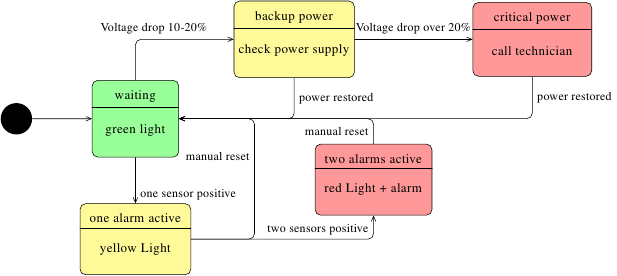
\includegraphics[scale=.6]{rad-warner-state.png}}
	 \note<.>{modelled stimuli+responses into states \\ here i modelled two sensor as a result of one sensor $\Rightarrow$ may be done differently}
\end{frame}

\begin{frame}{Programming language}
	\begin{itemize}
		\item program has to be\dots
		\note<.>{}the programming language \\ several things need to be taken into account \\ \ \\ program has to be
			\begin{itemize}
				\item \dots fast (i.e. C, Asssembler)
				\note<.>{\textbf{fast: C, Assembler:}\\ No concurrency \\ no built-in system for shared resources}
				\item \dots concurrent (i.e. C++, real time Java, \dots){}
				\note<.>{\textbf{concurrent:}\\ and manage shared resources}
			\end{itemize}
			\note<.>{\\ \ \\ \textbf{concurrent or speed??:}\\ depends on what is more important \\ simulate concurrency with frequent polling \\ do something yourself about shared resources}
			\item speed looses importance
			\note<.>{\textbf{speed:}\\ due to faster hardware \\ ie monitoring device written in C++ \\ ie cell phones in java, objective C, \dots \\ still there are some areas, where you need C \& assembler\dots}
			\item it's up to you in the end \dots
			\note<.>{it's up to you in the end\dots \\ evaluate the needs and decide\dots}
	\end{itemize}
\end{frame}

\section{Architectural patterns}
\begin{frame}{Architectural patterns}
	\begin{itemize}
		\item Architectural patterns are used to describe a system in an abstract way and help to understand the architecture.
		\note<.>{\textbf{note on the 3 patterns:}\\ The summerville book describes three rough design pattern \\ there are finer patterns that will lead to more exact design}
		\begin{itemize}
			\item Observe and react
			\note<.>{\textbf{Observe and React:}\\ set of monitored sensors \\ Something exeptional happens $\Rightarrow$ we do something \\ i.e. monitoring, incoming phone call}
			\item Environmental Control
			\note<.>{\textbf{Environmental Control:}\\ set of sensors and actuators \\ can change environment \\ i.e. flash light, when sensor fires \\i.e. control water level in a tank}
			\item Process Pipeline
			\note<.>{\textbf{Process Pipeline:}\\ data transformation \\ series of processing steps\\ preferably concurrent}
		\end{itemize}
		\note<.>{\\ \vspace*{1em} \textbf{all of those:} can be combined \\ often more than one pattern in the system \\ ie monitor the actuators}
		\note<.>{\ \\ \vspace*{1em} \textbf{design patterns:} will lead to \textbf{inefficient} system $\Rightarrow$ only for understanding system}
		\end{itemize}
\end{frame}

\begin{frame}{Observe and React}
	\begin{itemize}
		\item Observe and React
		\note<.>{Observer \& React}
		\begin{itemize}
			\item monitor the system with a set of sensors
			\note<.>{\textbf{monitoring:}\\ monitor the system with a set of sensors}
			\item display something
			\note<.>{\textbf{display:}\\ monitoring screen \\ on exceptional behaviour: alarms, shutdown\\ }
			\item primarly used in: Monitoring systems
			\note<.>{primarly in \textbf{monitoring systems:}\\ often consist of more than one O\&R patterns, one for each sensor \\ optimisation: combine something, ie display on one monitor}
		\end{itemize}
	\end{itemize}
\end{frame}

\begin{frame}{Environmental Control}
	\begin{itemize}
		\item Environmental Control
		\note<.>{Environmental Control}
		\begin{itemize}
			\item monitor the system and react to any changes
			\note<.>{monitor sytem and react to any changes}
			\item Used when there is no requirement for user interaction\dots{}
			\note<.>{no required user interaction \\ \textbf{examples:}\\ cruise control \\ water level \\ pressure control \\ \dots }
			\item \dots or no time for the user to interact \dots
			\note<.>{no time for user interaction \\ \textbf{examples:}\\ break assist \\ airbag}
			\item \dots no way a user can interact \dots{}
			\note<.>{no way for user interaction \\ \textbf{example:}\\ CYPRES {\tiny (parachute, Möllemann did not activate his in 2003)} \\ self desctruct of military/sensitive equipment}
			\item \dots or there is too much information for users to process.
			\note<.>{too much information for users \\ \textbf{example:}\\ Nuclear Power Plant \\ Airplane \\ Car \\ virtually any big system with many subsystems}
		\end{itemize}
	\end{itemize}
\end{frame}

\begin{frame}{Process Pipeline}
	\begin{itemize}
		\item Process Pipeline
		\begin{itemize}
			\item transform data
			\note<.>{transform data \\ \textbf{examples:}\\ signal processing from sensors in other systems \\ optical sensor \\ convert digital data to audio}
			\item often huge amounts of data to be converted in real time
			\note<.>{\textbf{huge amount in real time:}\\ concurrency + multicore is the key}
			\item data aquisition system: storing of data may need to be fast
			\note<.>{data aquisition system\textbf{example:}\\ particle accelerator \\ chemical reactions \\ \dots \\ if storing not fast, data will be lost}
		\end{itemize}
	\end{itemize}
\end{frame}

\section{Timing analysis}
\begin{frame}{Timing Analysis - I}
	\begin{itemize}
		\item timing analysis
		\note<.>{timing analysis}
		\begin{itemize}
			\item Correctness of systems depends not only on result, but also on the time at which the result is produced.
			\note<.>{not only result, also time is important \\ soft and hard systems}
			\item How often does each process need to be executed?
			\note<.>{\textbf{how often?:}\\ then we check, if our system can deliver this \\ this can be quite hard, when \emph{mixture of aperiodic and periodic stimuli} or \emph{many aperiodic stimuli} are expected}
			\item aperiodic stimuly $\Rightarrow$ make assumptions
			\note<.>{\textbf{aperiodic stimuli:} \\ make assumptions}
			\note<.>{\\ vspace*{1em} \textbf{fast systems:}\\ use only periodic stimuli \\ poll frequently for aperiodic stimuli}
		\end{itemize}
	\end{itemize}
\end{frame}

\begin{frame}{Timing Analysis - II}
	\begin{itemize}
		\item Consider:
		\note<.>{Timing analysis must consider:}
		\begin{itemize}
			\item deadlines
			\note<.>{\textbf{deadlines:}\\ By which time must the process have ended.}
			\item frequency
			\note<.>{\textbf{frequency:}\\ The number of times a process must be executed in a given span, so that the \emph{system} meets all deadlines}
			\item execution time
			\note<.>{\textbf{execution time:}\\ How long does each single process take (average \& worst case) \\ hard: conditional execution, delays waiting, \dots \\ \textbf{hard systems:} always worst case}
		\end{itemize}
	\end{itemize}
\end{frame}

\begin{frame}
\setbeamercovered{invisible}
	\begin{tabular}{p{9em}p{13em}}
		\rowcolor{structure.fg}\hline \textcolor{white}{Stimulus/Response} & \textcolor{white}{Timing requirements} \pause \\
		voltage drop & switch to backup: 50ms \pause \\
		sensor reaction & poll twice a second \pause \\
		turn on light & 500ms \pause \\
		call technician & 5000ms \\
	\end{tabular}
	\note<1>{We list stimuli and response \\ then think about how fast this needs to work}
	\note<2>{voltage drop $\Rightarrow$ 50ms}
	\note<3>{sensor reaction $\Rightarrow$ poll twice a second}
	\note<4>{turn on light $\Rightarrow$ 500ms}
	\note<5>{call technician $\Rightarrow$ 5000ms \\ may take longer, as technician reaction time is low anyways}
	\note<5>{\textbf{LAST CELL:}\\}
\setbeamercovered{transparent=25}
\end{frame}

\section{Real-time operating systems}
\begin{frame}{Real-time operating systems}
	\begin{itemize}
		\item normal operating systems not feasible
		\note<.>{\textbf{normal operating systems:}\\ too large, too bulky, too slow}
		\item special ``real-time operating systems'' exist
		\note<.>{\textbf{real-time operating systems:}\\Windows/CE \\ Vxworks \\ RTLinux \\ emdebian\\ \ \\ they are small and damn fast}
		\item RTOS must include:
		\note<.>{RTOS must include}
		\begin{itemize}
			\item real-time clock
			\note<.>{\textbf{real-time clock:}\\ provides information required to schedule processes}
			\item interrupt handler
			\note<.>{\textbf{interrupt handler:}\\ manages aperiodic requests for service \\ may be inside process manager \\ at least \textbf{2 levels:} \\ \emph{interrupt} for processes with fast response time \& \emph {clock level} fore regular processes \\ often also background processes with low priority {\tiny (self checks etc)}}
			\item process manager: scheduler \& resource manager
			\note<.>{\textbf{scheduler}\\ examines processes and chooses one for execution \\ processes need enough processor time to \emph{finish before their deadline} \\ \textbf{commonly used:} \\ non-pre-emptive \& pre-emtive (execution of processes may be stopped) \\ \emph{round robin} \\ rate monolithic scheduling (SJF) \\ shortes deadline first (HPF) }
			\note<.>{\\ \textbf{resource manager:}\\ allocates memory and processor resources scheduled for execution}
			\item dispatcher
			\note<.>{\textbf{dispatcher:}\\ starts execution of processes}
		\end{itemize}
	\end{itemize}
\end{frame}

\begin{frame}{30 minutes in short}
	\begin{itemize}
		\item What you should (at least) remember:
		\note<.>{nearly done \\ important stuff in short}
		\begin{itemize}
			\item Embedded Systems react to events in real time.
			\note<.->{\textbf{Embedded Systems} \\ react to events in real time}
			\item Embedded Systems are a set of processes reacting to stimuli
			\note<.->{\\ are a set of processes reacting to stimuli}
			\item State models help understanding the System.
			\note<.->{\\ \textbf{state models}\\ help understanding the system}
			\item Architectural patterns can be used to help in designing the system.
			\note<.->{\textbf{Architectural patterns} \\ help designing the system {\tiny especially first steps}}
			\item Always do timing analysis in (hard) Embedded Systems.
			\note<.->{timing analysis must always be done in (hard) systems}
		\end{itemize}
	\end{itemize}
\end{frame}

\begin{frame}[c]
\frametitle{Questions?}
	\centerline{\Huge Questions?}
\end{frame}

\end{document}
